\documentclass{article}
\usepackage{xcolor}
\usepackage{titleps}
\usepackage[letterpaper, margin=0.95in]{geometry}
\usepackage{url}
\usepackage{amsmath}
\usepackage{amssymb}
\usepackage{wrapfig}
\usepackage{float}
\usepackage{mathtools}
\usepackage{enumitem}
\usepackage{tabu}
\usepackage{parskip}
\usepackage{natbib}
\usepackage{listings}

\usepackage[many]{tcolorbox}
\usepackage{minted}
\setminted[python]{
	% frame=single,
	% linenos,
    xleftmargin=0.475em,
    baselinestretch=1.2,
}
% https://tex.stackexchange.com/a/569249
\setcounter{secnumdepth}{5}
\setcounter{tocdepth}{5}
\makeatletter
\newcommand\subsubsubsection{\@startsection{paragraph}{4}{\z@}{-2.5ex\@plus -1ex \@minus -.25ex}{1.25ex \@plus .25ex}{\normalfont\normalsize\bfseries}}
\newcommand\subsubsubsubsection{\@startsection{subparagraph}{5}{\z@}{-2.5ex\@plus -1ex \@minus -.25ex}{1.25ex \@plus .25ex}{\normalfont\normalsize\bfseries}}
\makeatother

\usepackage{hyperref}
\usepackage[color=red]{todonotes}
\usepackage{forest}
\definecolor{light-yellow}{HTML}{FFE5CC}

\newpagestyle{ruled}
{\sethead{CMU 16-831}{Introduction to Robot Learning }{Fall 2024}\headrule
  \setfoot{}{}{}}
\pagestyle{ruled}

\renewcommand\makeheadrule{\color{black}\rule[-.75\baselineskip]{\linewidth}{0.4pt}}
\renewcommand*\footnoterule{}

\newtcolorbox[]{answer}[1][]{
    % breakable,
    enhanced,
    nobeforeafter,
    colback=white,
    title=Your Answer,
    sidebyside align=top,
    box align=top,
    #1
}



\begin{document}

\lstset{basicstyle = \ttfamily,columns=fullflexible,
    backgroundcolor = \color{light-yellow}
}

\begin{centering}
    {\Large Assignment 2: Policy Gradient} \\
    \vspace{.25cm}
    % \textbf{Due September 13, 11:59 pm} \\
\end{centering}
\vspace{0.25cm}

\textbf{Andrew ID:} \texttt{mukaiy} \\
% \textbf{Collaborators:} \texttt{Write the Andrew IDs of your collaborators here (if any).}\\
\textbf{NOTE:} Please do \textbf{NOT} change the sizes of the answer blocks or plots.

\setcounter{section}{4}
\section{Small-Scale Experiments}

\subsection{Experiment 1 (Cartpole) -- \lbrack25 points total\rbrack}

\subsubsection{Configurations}
\begin{answer}[title=Q5.1.1,height=6cm,width=\linewidth]
    % TODO
    \begin{minted}
[framesep=2mm, fontsize=\scriptsize, breaklines]
{bash}
python rob831/scripts/run_hw2.py --env_name CartPole-v0 -n 100 -b 1000 \
    -dsa --exp_name q1_sb_no_rtg_dsa

python rob831/scripts/run_hw2.py --env_name CartPole-v0 -n 100 -b 1000 \
    -rtg -dsa --exp_name q1_sb_rtg_dsa

python rob831/scripts/run_hw2.py --env_name CartPole-v0 -n 100 -b 1000 \
    -rtg --exp_name q1_sb_rtg_na

python rob831/scripts/run_hw2.py --env_name CartPole-v0 -n 100 -b 5000 \
    -dsa --exp_name q1_lb_no_rtg_dsa

python rob831/scripts/run_hw2.py --env_name CartPole-v0 -n 100 -b 5000 \
    -rtg -dsa --exp_name q1_lb_rtg_dsa

python rob831/scripts/run_hw2.py --env_name CartPole-v0 -n 100 -b 5000 \
    -rtg --exp_name q1_lb_rtg_na
\end{minted}
\end{answer}

\subsubsection{Plots}

\subsubsubsection{Small batch -- \lbrack5 points\rbrack}
\begin{answer}[title=Q5.1.2.1,height=9.5cm,width=\linewidth]
    % TODO
    \centering
    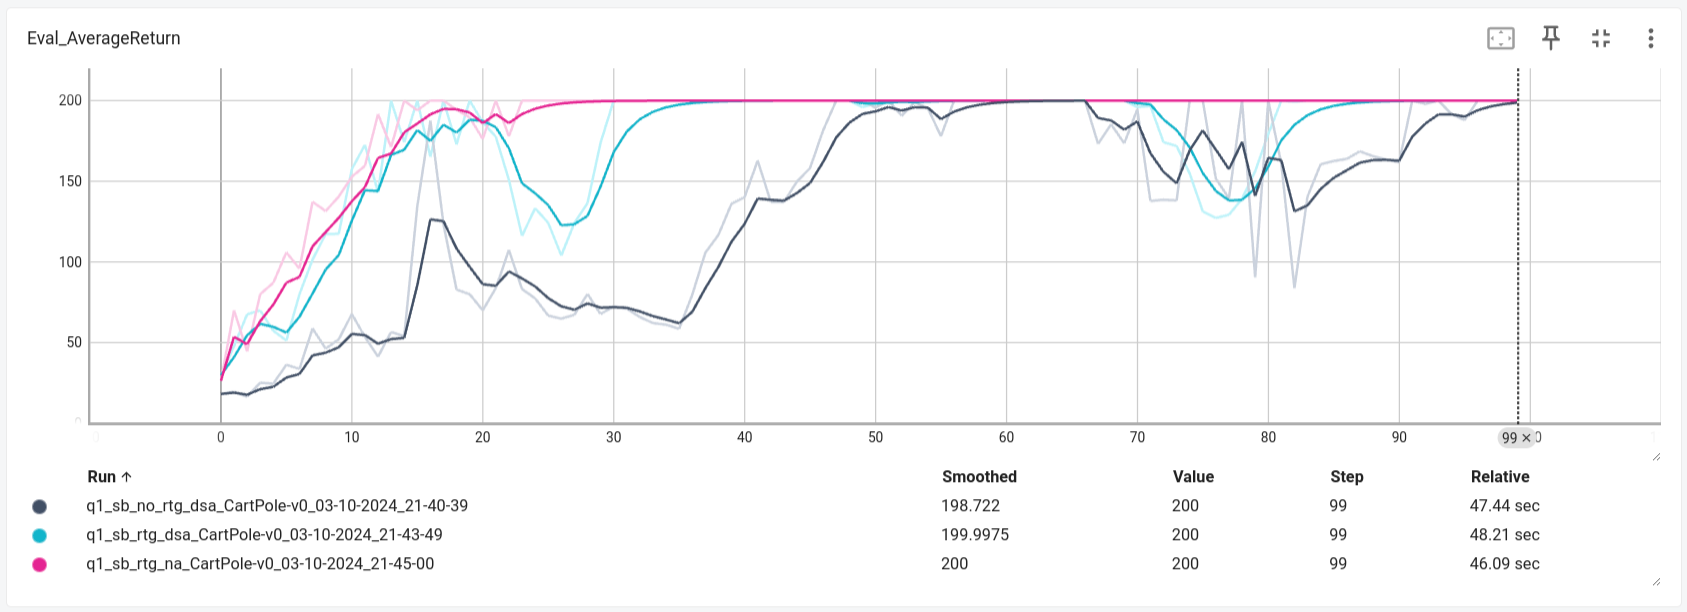
\includegraphics[width=.99\linewidth]{figs/Q5_small_batch.png}
\end{answer}

\subsubsubsection{Large batch -- \lbrack5 points\rbrack}
\begin{answer}[title=Q5.1.2.2,height=9.5cm,width=\linewidth]
    % TODO
    \centering
    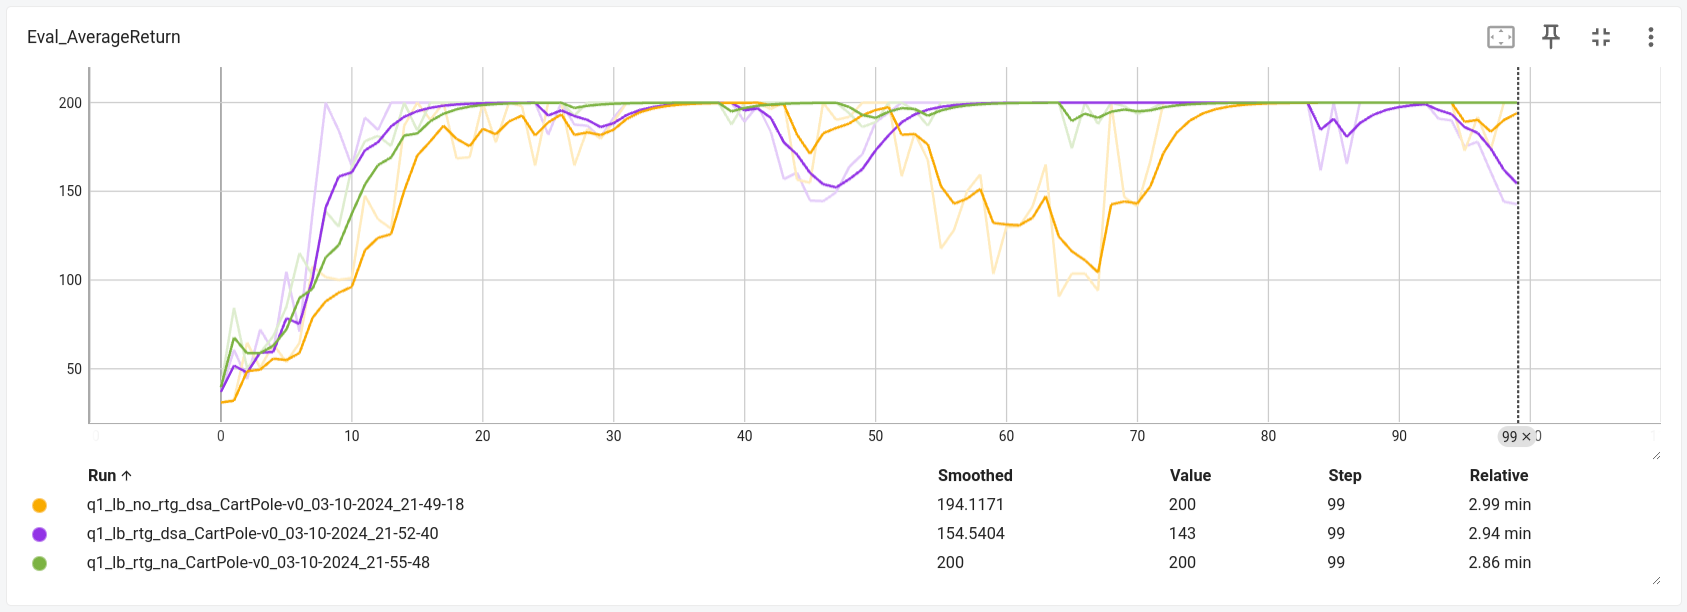
\includegraphics[width=.99\linewidth]{figs/Q5_large_batch.png}
\end{answer}

\subsubsection{Analysis}

\subsubsubsection{Value estimator -- \lbrack5 points\rbrack}
\begin{answer}[title=Q5.1.3.1,height=4cm,width=\linewidth]
    Obviously reward-to-go because of causality and smaller variance.
\end{answer}

\subsubsubsection{Advantage standardization -- \lbrack5 points\rbrack}
\begin{answer}[title=Q5.1.3.2,height=4cm,width=\linewidth]
    Yes, it does help.
    It helps to stabilize the learning process by reducing the variance of the advantage estimates.

    One thing I don't understand is why changing the bias has no significant impact on training, since standardization changes the mean.
    Each reward is a function of both state and action, so moving the mean shouldn't be just like adding a state-dependent bias, e.g., $V(s)$, right?

    I guess it's because this process only "slightly" biases the advantage estimates, pretty much like the effect of not having accurate $V(s)$ in the actor-critic method.
\end{answer}

\subsubsubsection{Batch size -- \lbrack5 points\rbrack}
\begin{answer}[title=Q5.1.3.3,height=4cm,width=\linewidth]
    I would say that batch size marginally helps to improve the policy faster, and I think the improvement is non-linear, which is why we don't see the time-to-plateau gets $\frac{1}{5}$ed.

    But more data does help the experiment without reward-to-go to converge faster, since it typically needs more rollouts, i.e., more state/action/reward tuples, because it typically has higher variance.
\end{answer}

\subsection{Experiment 2 (InvertedPendulum) -- \lbrack15 points total\rbrack}

\subsubsection{Configurations -- \lbrack5 points\rbrack}
\begin{answer}[title=Q5.2.1,height=10cm,width=\linewidth]
    % TODO
    \begin{minted}
[framesep=2mm, fontsize=\scriptsize, breaklines]
{bash}
python rob831/scripts/run_hw2.py --env_name InvertedPendulum-v4 \
    --ep_len 1000 --discount 0.9 -n 100 -l 2 -s 64 -b 10000 -lr 0.001 -rtg \
    --exp_name q2_b_10000_r_0.001

python rob831/scripts/run_hw2.py --env_name InvertedPendulum-v4 \
    --ep_len 1000 --discount 0.9 -n 100 -l 2 -s 64 -b 1000 -lr 0.001 -rtg \
    --exp_name q2_b_1000_r_0.001

python rob831/scripts/run_hw2.py --env_name InvertedPendulum-v4 \
    --ep_len 1000 --discount 0.9 -n 100 -l 2 -s 64 -b 1000 -lr 0.01 -rtg \
    --exp_name q2_b_1000_r_0.01

python rob831/scripts/run_hw2.py --env_name InvertedPendulum-v4 \
    --ep_len 1000 --discount 0.9 -n 100 -l 2 -s 64 -b 1000 -lr 0.05 -rtg \
    --exp_name q2_b_1000_r_0.05

python rob831/scripts/run_hw2.py --env_name InvertedPendulum-v4 \
    --ep_len 1000 --discount 0.9 -n 100 -l 2 -s 64 -b 1000 -lr 0.1 -rtg \
    --exp_name q2_b_1000_r_0.1

python rob831/scripts/run_hw2.py --env_name InvertedPendulum-v4 \
    --ep_len 1000 --discount 0.9 -n 100 -l 2 -s 64 -b 100 -lr 0.1 -rtg \
    --exp_name q2_b_100_r_0.1

python rob831/scripts/run_hw2.py --env_name InvertedPendulum-v4 \
    --ep_len 1000 --discount 0.9 -n 100 -l 2 -s 64 -b 2000 -lr 0.01 -rtg \
    --exp_name q2_b_2000_r_0.01

python rob831/scripts/run_hw2.py --env_name InvertedPendulum-v4 \
    --ep_len 1000 --discount 0.9 -n 100 -l 2 -s 64 -b 500 -lr 0.01 -rtg \
    --exp_name q2_b_500_r_0.01

python rob831/scripts/run_hw2.py --env_name InvertedPendulum-v4 \
    --ep_len 1000 --discount 0.9 -n 100 -l 2 -s 64 -b 800 -lr 0.01 -rtg \
    --exp_name q2_b_800_r_0.01
\end{minted}
\end{answer}

\subsubsection{smallest \textbf{b*} and largest \textbf{r*} (same run) -- \lbrack5 points\rbrack}
\begin{answer}[title=Q5.2.2,height=4cm,width=\linewidth]
    % TODO
    b* = 500

    r* = 0.01
\end{answer}

\subsubsection{Plot -- \lbrack5 points\rbrack}
\begin{answer}[title=Q5.2.3,height=10cm,width=\linewidth]
    % TODO
    \centering
    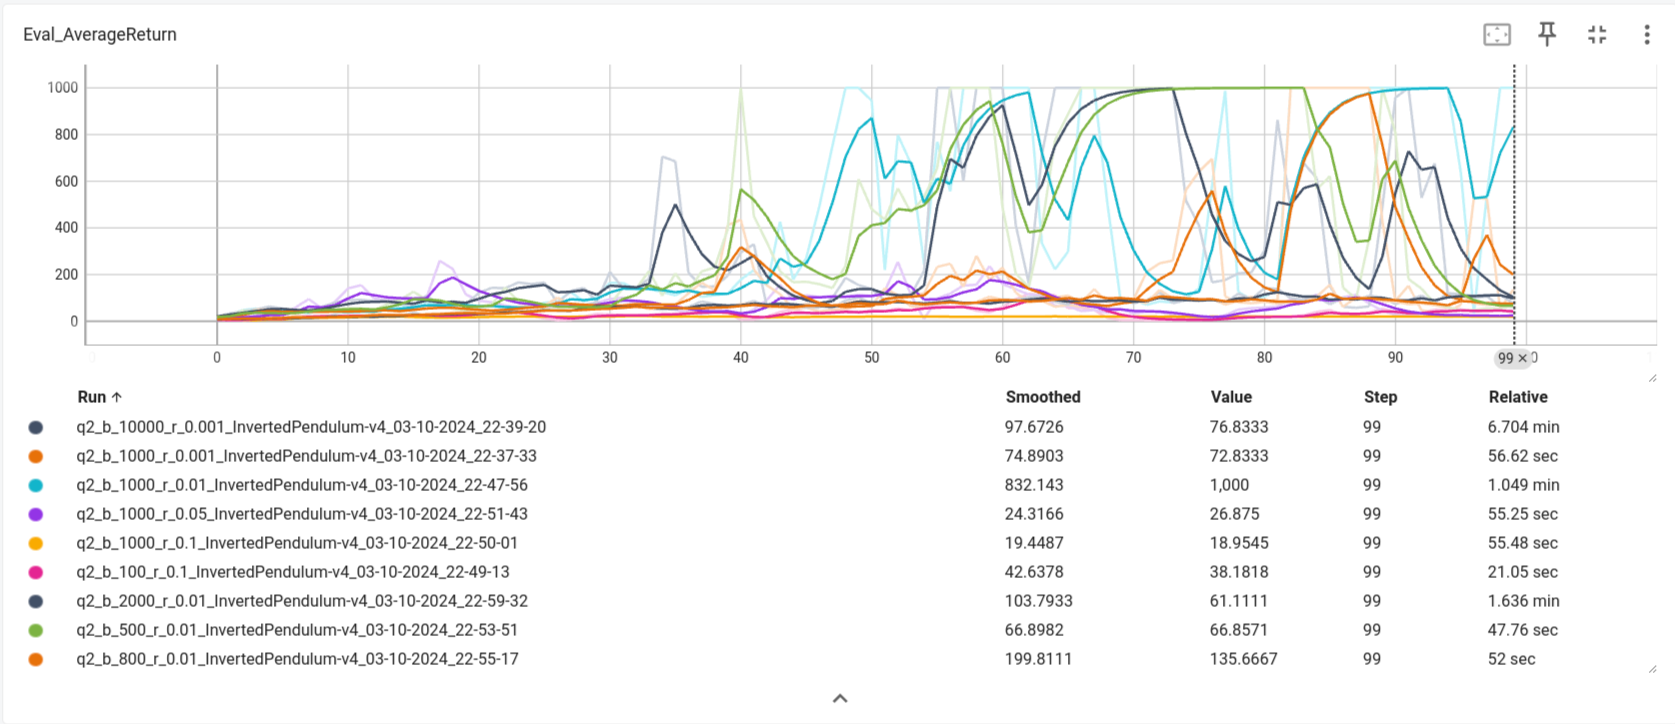
\includegraphics[width=.99\linewidth]{figs/Q5_exp_2.png}
\end{answer}

\setcounter{section}{6}
\section{More Complex Experiments}

\subsection{Experiment 3 (LunarLander) -- \lbrack10 points total\rbrack}

\subsubsection{Configurations}
\begin{answer}[title=Q7.1.1,height=6cm,width=\linewidth]
    \begin{minted}
[framesep=2mm, fontsize=\scriptsize, breaklines]
{bash}
python rob831/scripts/run_hw2.py \
    --env_name LunarLanderContinuous-v4 --ep_len 1000 \
    --discount 0.99 -n 100 -l 2 -s 64 -b 10000 -lr 0.005 \
    --reward_to_go --nn_baseline --exp_name q3_b10000_r0.005
\end{minted}
\end{answer}

\subsubsection{Plot -- \lbrack10 points\rbrack}
\begin{answer}[title=Q7.1.2,height=10cm,width=\linewidth]
    % TODO
    \centering
    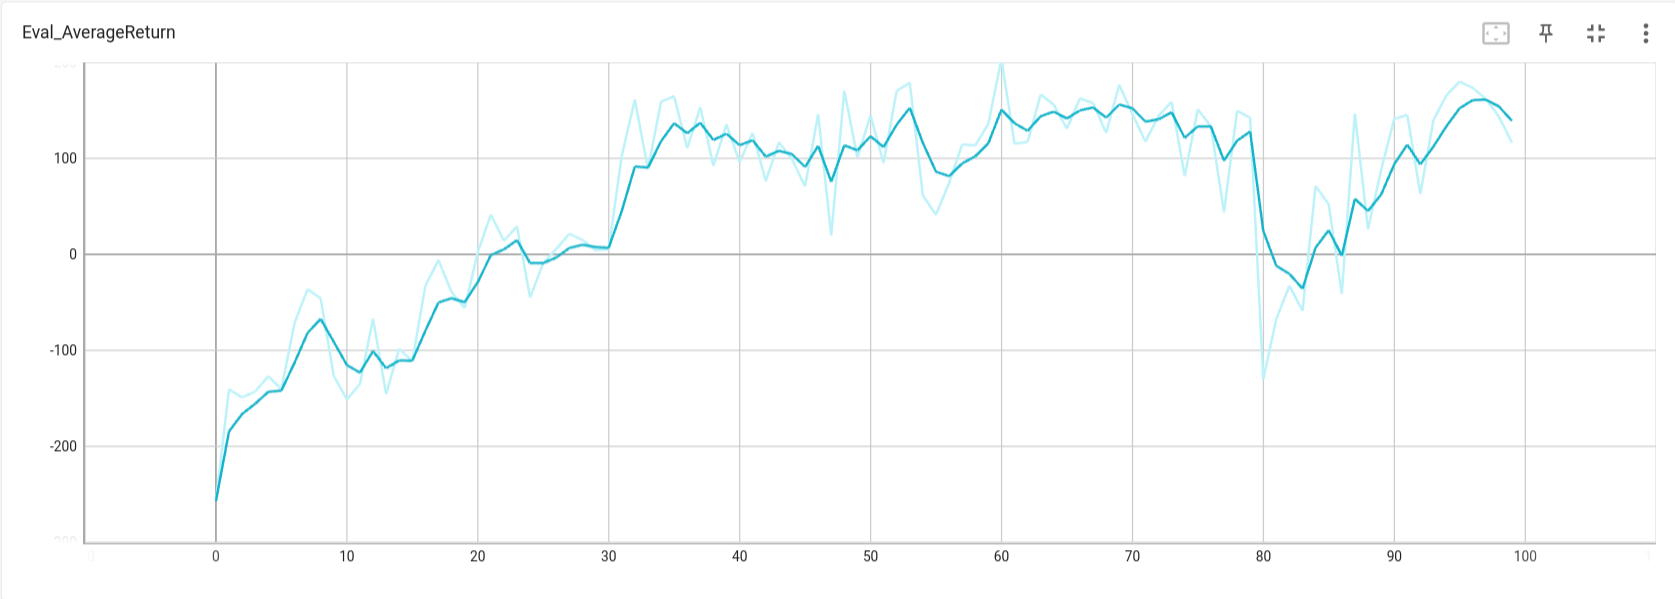
\includegraphics[width=.99\linewidth]{figs/Q7_lunar_lander.png}
\end{answer}

\subsection{Experiment 4 (HalfCheetah) -- \lbrack30 points\rbrack}

\subsubsection{Configurations}
\begin{answer}[title=Q7.2.1,height=10cm,width=\linewidth]
    \begin{minted}
[framesep=2mm, fontsize=\scriptsize, breaklines, escapeinside=||, mathescape=true]
{python}
python rob831/scripts/run_hw2.py --env_name HalfCheetah-v4 --ep_len 150 \
    --discount 0.95 -n 100 -l 2 -s 32 -b 10000 -lr 0.02 \
    --exp_name q4_search_b10000_lr0.02
python rob831/scripts/run_hw2.py --env_name HalfCheetah-v4 --ep_len 150 \
    --discount 0.95 -n 100 -l 2 -s 32 -b 30000 -lr 0.02 -rtg \
    --exp_name q4_search_b30000_lr0.02_rtg
python rob831/scripts/run_hw2.py --env_name HalfCheetah-v4 --ep_len 150 \
    --discount 0.95 -n 100 -l 2 -s 32 -b 50000 -lr 0.02 --nn_baseline \
    --exp_name q4_search_b50000_lr0.02_nnbaseline
python rob831/scripts/run_hw2.py --env_name HalfCheetah-v4 --ep_len 150 \
    --discount 0.95 -n 100 -l 2 -s 32 -b 10000 -lr 0.01 \
    --exp_name q4_search_b10000_lr0.01
python rob831/scripts/run_hw2.py --env_name HalfCheetah-v4 --ep_len 150 \
    --discount 0.95 -n 100 -l 2 -s 32 -b 30000 -lr 0.01 -rtg \
    --exp_name q4_search_b30000_lr0.01_rtg
python rob831/scripts/run_hw2.py --env_name HalfCheetah-v4 --ep_len 150 \
    --discount 0.95 -n 100 -l 2 -s 32 -b 50000 -lr 0.01 --nn_baseline \
    --exp_name q4_search_b50000_lr0.01_nnbaseline
python rob831/scripts/run_hw2.py --env_name HalfCheetah-v4 --ep_len 150 \
    --discount 0.95 -n 100 -l 2 -s 32 -b 10000 -lr 0.005 \
    --exp_name q4_search_b10000_lr0.005
python rob831/scripts/run_hw2.py --env_name HalfCheetah-v4 --ep_len 150 \
    --discount 0.95 -n 100 -l 2 -s 32 -b 30000 -lr 0.005 -rtg \
    --exp_name q4_search_b30000_lr0.005_rtg
python rob831/scripts/run_hw2.py --env_name HalfCheetah-v4 --ep_len 150 \
    --discount 0.95 -n 100 -l 2 -s 32 -b 50000 -lr 0.005 --nn_baseline \
    --exp_name q4_search_b50000_lr0.005_nnbaseline
\end{minted}
\end{answer}

\subsubsection{Plot -- \lbrack10 points\rbrack}
\begin{answer}[title=Q7.2.2,height=10cm,width=\linewidth]
    % TODO
    \begin{figure}[H]
        \centering
        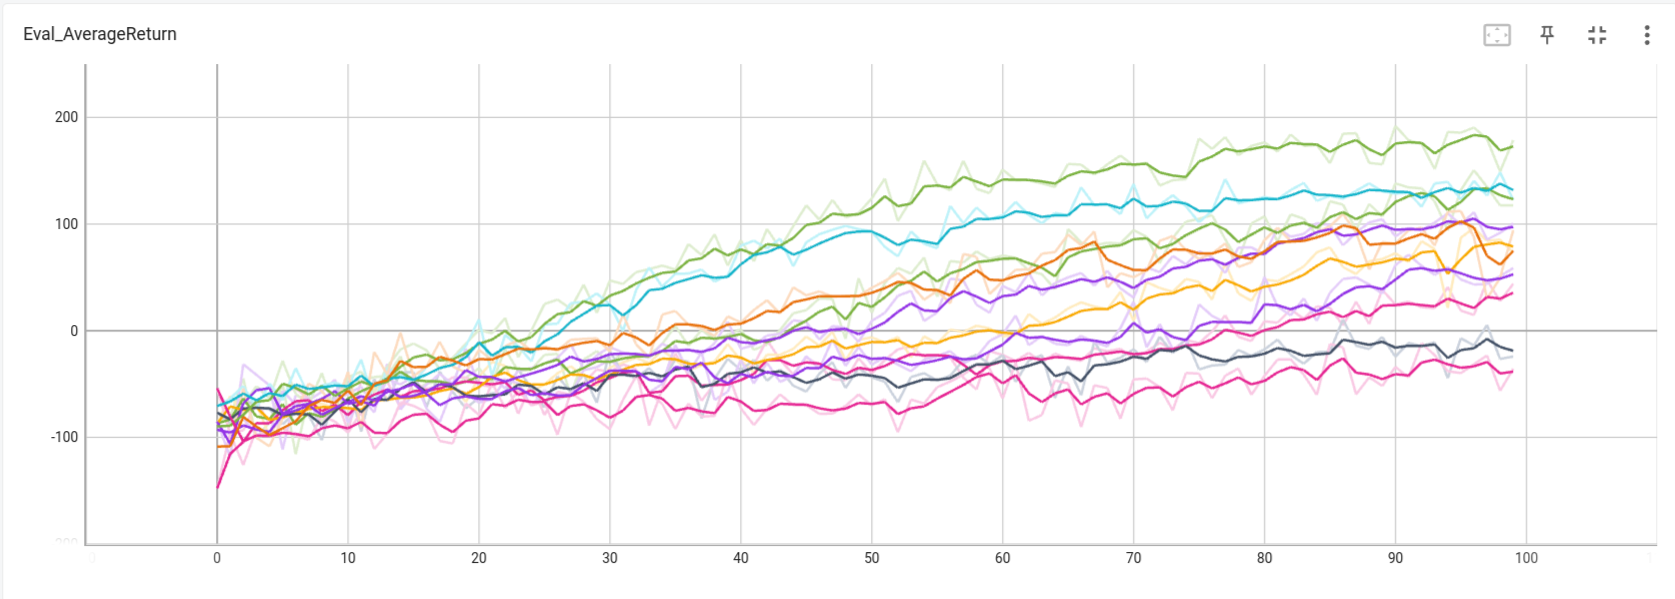
\includegraphics[width=.99\linewidth]{figs/Q7_half_cheetah_all.png}
        \caption{Brute-force search for the best batch size and learning rate}
    \end{figure}
\end{answer}

\subsubsection{(Optional) Optimal b* and r* -- \lbrack3 points\rbrack}
\begin{answer}[title=Q7.2.3,height=4cm,width=\linewidth]
    % TODO
    b* = 50000

    r* = 0.02
\end{answer}

\subsubsection{(Optional) Plot -- \lbrack10 points\rbrack}
\begin{answer}[title=Q7.2.4,height=10cm,width=\linewidth]
    % TODO
    \begin{figure}[H]
        \centering
        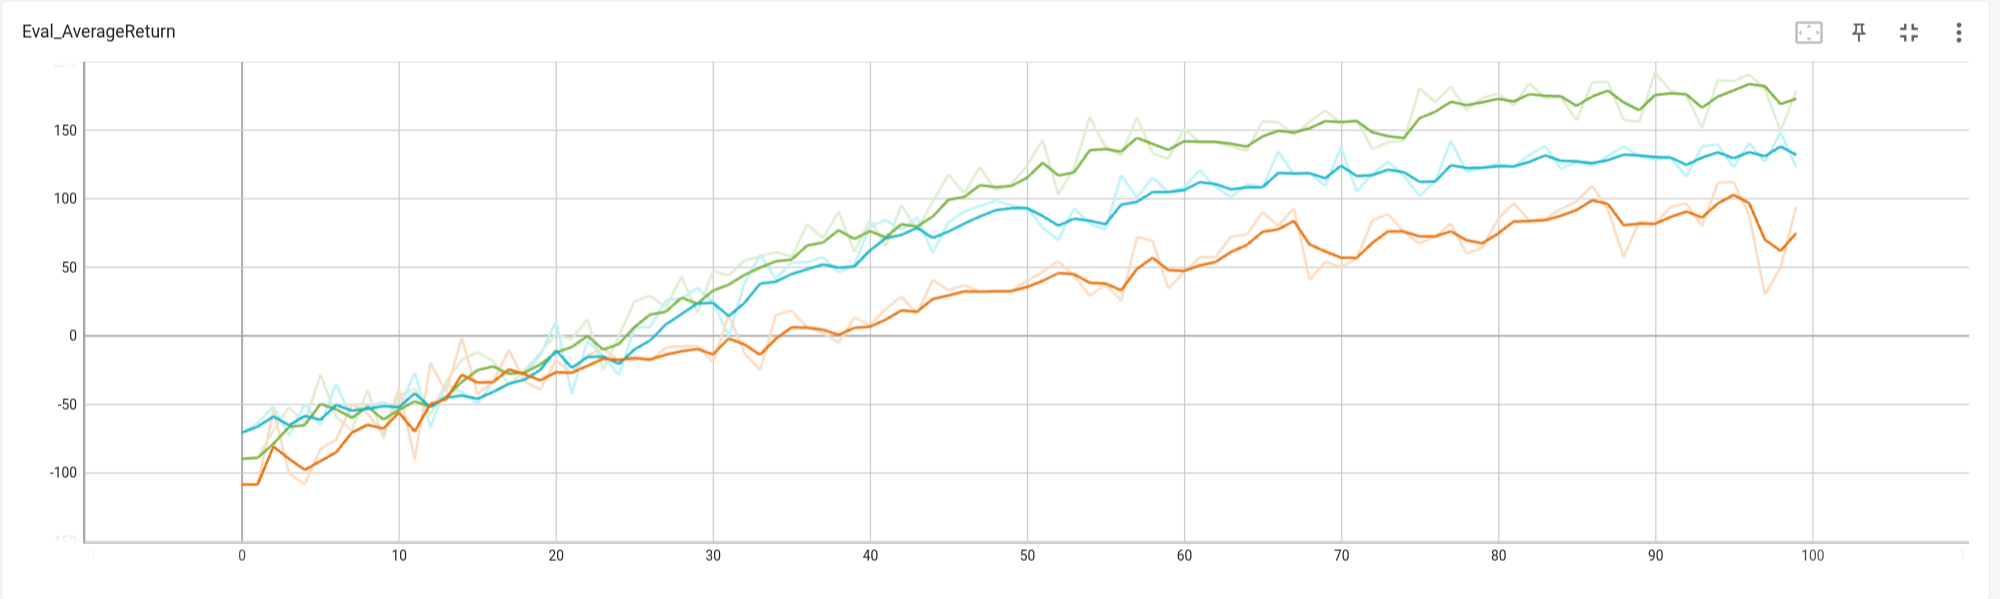
\includegraphics[width=.99\linewidth]{figs/Q7_half_cheetah_large_lr.png}
        \caption{Learning rate = 0.02}
    \end{figure}
\end{answer}

\subsubsection{(Optional) Describe how b* and r* affect task performance -- \lbrack7 points\rbrack}
\begin{answer}[title=Q7.2.5,height=4cm,width=\linewidth]
    % TODO
    First of all, there's still rooms for improvement if we train more iterations.

    Larger batch and learning rate help to improve the policy faster.

    I personally thinks learning rate affects more because all the configurations with learning rate = 0.02 achieved above 0 evaluation average return.
\end{answer}

\subsubsection{(Optional) Configurations with optimal b* and r* -- \lbrack3 points\rbrack}
\begin{answer}[title=Q7.2.6,height=6cm,width=\linewidth]
    % TODO
    \begin{minted}
[framesep=2mm, fontsize=\scriptsize, breaklines]
{bash}
python rob831/scripts/run_hw2.py --env_name HalfCheetah-v4 --ep_len 150 \
    --discount 0.95 -n 100 -l 2 -s 32 -b 50000 -lr 0.02 \
    --exp_name q4_b50000_r0.02

python rob831/scripts/run_hw2.py --env_name HalfCheetah-v4 --ep_len 150 \
    --discount 0.95 -n 100 -l 2 -s 32 -b 50000 -lr 0.02 -rtg \
    --exp_name q4_b50000_r0.02_rtg

python rob831/scripts/run_hw2.py --env_name HalfCheetah-v4 --ep_len 150 \
    --discount 0.95 -n 100 -l 2 -s 32 -b 50000 -lr 0.02 --nn_baseline \
    --exp_name q4_b50000_r0.02_nnbaseline

python rob831/scripts/run_hw2.py --env_name HalfCheetah-v4 --ep_len 150 \
    --discount 0.95 -n 100 -l 2 -s 32 -b 50000 -lr 0.02 -rtg --nn_baseline \
    --exp_name q4_b50000_r0.02_rtg_nnbaseline
\end{minted}
\end{answer}

\subsubsection{(Optional) Plot for four runs with optimal b* and r* -- \lbrack7 points\rbrack}
\begin{answer}[title=Q7.2.7,height=10cm,width=\linewidth]
    % TODO
    \begin{figure}[H]
        \centering
        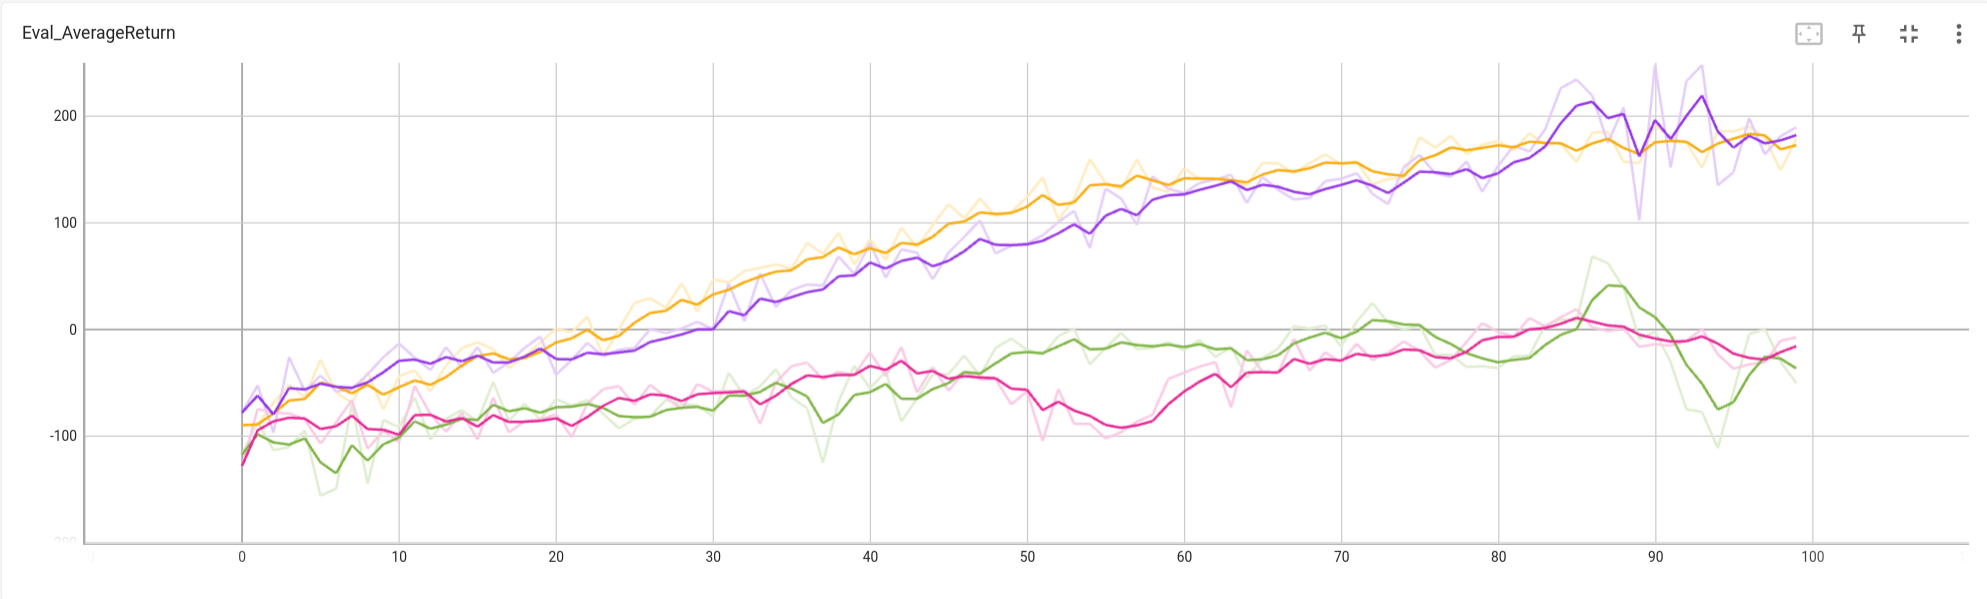
\includegraphics[width=.99\linewidth]{figs/Q7_half_cheetah_optimal.png}
        \caption{\textcolor{orange}{orange: rtg + baseline}, \textcolor{violet}{violet: rtg}, \textcolor{magenta}{magenta: baseline}, \textcolor{green}{green: nothing}}
    \end{figure}

    Reward-to-go boosts so much.
\end{answer}

\section{Implementing Generalized Advantage Estimation}

\subsection{Experiment 5 (Hopper) -- \lbrack20 points\rbrack}

\subsubsection{Configurations}
\begin{answer}[title=Q8.1.1,height=4cm,width=\linewidth]
    \begin{minted}
[framesep=2mm, fontsize=\scriptsize, breaklines, escapeinside=||, mathescape=true]
{python}
# $\lambda \in [0,0.95,0.99,1]$
python rob831/scripts/run_hw2.py \
    --env_name Hopper-v4 --ep_len 1000 \
    --discount 0.99 -n 300 -l 2 -s 32 -b 2000 -lr 0.001 \
    --reward_to_go --nn_baseline --action_noise_std 0.5 --gae_lambda <|$\lambda$|> \
    --exp_name q5_b2000_r0.001_lambda<|$\lambda$|>
\end{minted}
\end{answer}

\subsubsection{Plot -- \lbrack13 points\rbrack}
\begin{answer}[title=Q8.1.2,height=10cm,width=\linewidth]
    % TODO
    \begin{figure}[H]
        \centering
        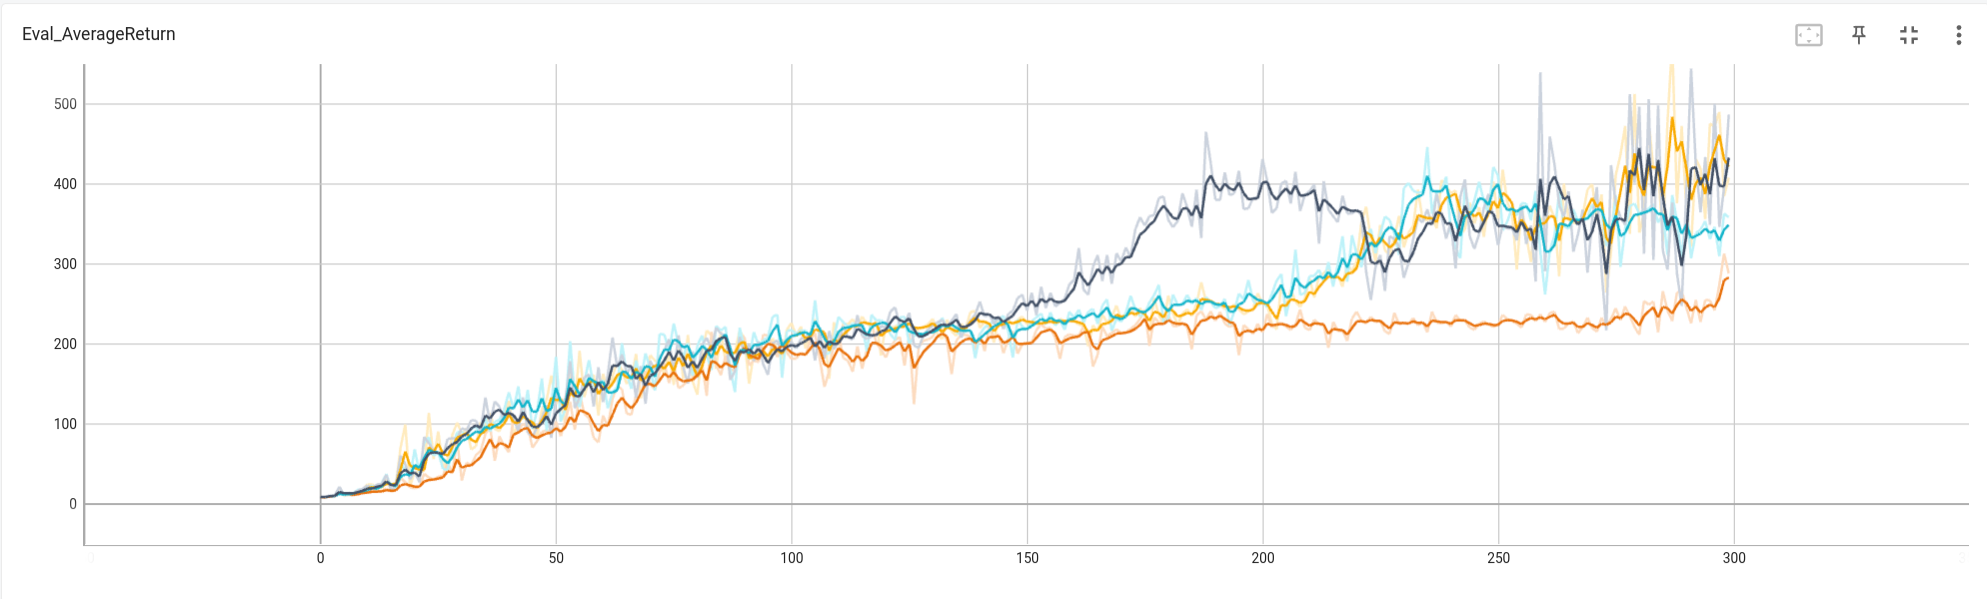
\includegraphics[width=.99\linewidth]{figs/Q8.png}
        \caption{\textcolor{black}{black: $\lambda = 0.95$}, \textcolor{yellow}{yellow: $\lambda = 1$}, \textcolor{cyan}{cyan: $\lambda = 0.99$, \textcolor{orange}{orange: $\lambda = 0$}}}
    \end{figure}
\end{answer}

\subsubsection{Describe how $\lambda$ affects task performance -- \lbrack7 points\rbrack}
\begin{answer}[title=Q8.1.3,height=4cm,width=\linewidth]
    % TODO
    Lower $\lambda$ values means we trust each individual rollouts over the value function (baseline), which typically has higher variance, or more noise.

    Higher $\lambda$ values means the opposite.

    GAE's pretty clever in that it maps the input from $n \in [0, T - t - 1]$ to $\lambda \in [0, 1]$, so $\lambda$ is basically the percentage of how much remaining rollouts to use, and how much we trust the reward-to-go.
    But it's non-linear, which is probably why we need to optimize around [0.9, 1]
\end{answer}

\clearpage

\section{Bonus! (optional)}

\subsection{Parallelization -- \lbrack15 points\rbrack}
\begin{answer}[title=Q9.1,height=20cm,width=\linewidth]
    % TODO (optional)
    \begin{figure}[H]
        \centering
        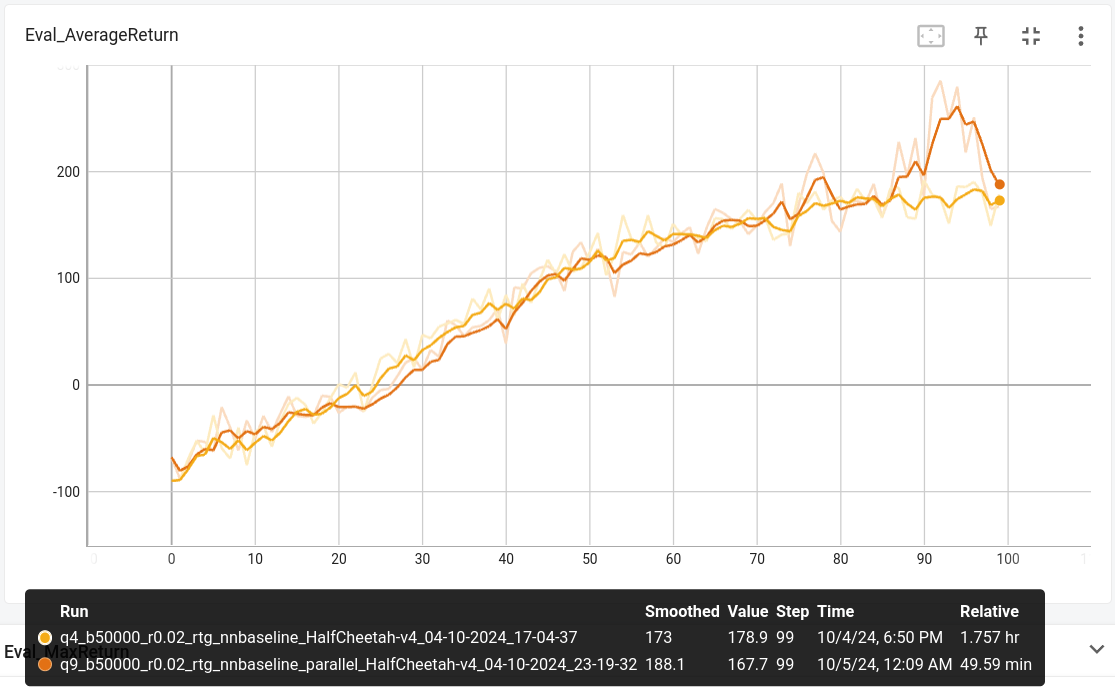
\includegraphics[width=.99\linewidth]{figs/Q9_parallelization.png}
    \end{figure}
    num\_worker\_threads is adaptive according to $\frac{\text{min\_timesteps\_per\_batch}}{\text{average\_path\_length}}$, capped by mp.cpu\_count() - 1
    I'm training on a laptop with 32 CPU hardware threads.

    Difference in training time:
    $\frac{1.757 \text{hr}}{49.59 \text{min}} \approx 2$
    \vspace{1.0cm}
    \begin{minted}
[framesep=2mm, fontsize=\scriptsize, breaklines, escapeinside=||, mathescape=true]
{python}
python rob831/scripts/run_hw2.py --env_name HalfCheetah-v4 --ep_len 150 \
    --discount 0.95 -n 100 -l 2 -s 32 -b 50000 -lr 0.02 -rtg --nn_baseline --parallel \
    --exp_name q9_b50000_r0.02_rtg_nnbaseline_parallel
\end{minted}
\end{answer}

\subsection{Multiple gradient steps -- \lbrack5 points\rbrack}
\begin{answer}[title=Q9.1,height=20cm,width=\linewidth]
    % TODO (optional)
    \begin{figure}[H]
        \centering
        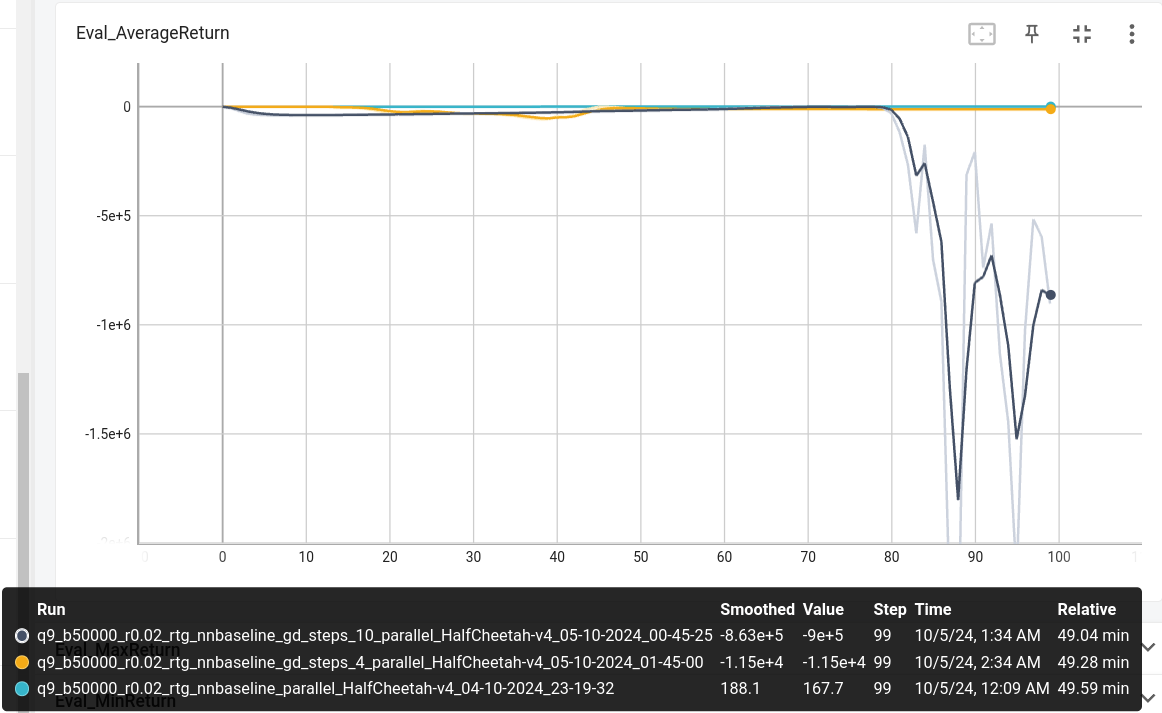
\includegraphics[width=.99\linewidth]{figs/Q9_multi_gd_step.png}
    \end{figure}
    Basically on-policy vs off-policy, off-policy without re-evaluating the policy to get up-to-date action and reward will result in negative effects.

    Even if actions and rewards are re-evaluated after each gradient step, $p_\theta(s)$ still won't change, resulting in a larger exploration space, which makes the policy more robust (covers wider range) but less optimized (for the states it's supposed to optimize).
    \vspace{1.0cm}
    \begin{minted}
[framesep=2mm, fontsize=\scriptsize, breaklines]
{bash}
python rob831/scripts/run_hw2.py --env_name HalfCheetah-v4 --ep_len 150 \
    --discount 0.95 -n 100 -l 2 -s 32 -b 50000 -lr 0.02 -rtg --nn_baseline --parallel --num_agent_train_steps_per_iter 4 \
    --exp_name q9_b50000_r0.02_rtg_nnbaseline_gd_steps_4_parallel

python rob831/scripts/run_hw2.py --env_name HalfCheetah-v4 --ep_len 150 \
    --discount 0.95 -n 100 -l 2 -s 32 -b 50000 -lr 0.02 -rtg --nn_baseline --parallel --num_agent_train_steps_per_iter 10 \
    --exp_name q9_b50000_r0.02_rtg_nnbaseline_gd_steps_10_parallel
\end{minted}

\end{answer}

\end{document}
